\documentclass[12pt]{article}
\usepackage{latexblog}

% ============================================================
% Blog Metadata
% ============================================================
\blogtitle{关于代码注释}
\blogdate{2018-01-16}
\blogtags{开发实践, 闲话编程}
\bloglang{zh}
\blogsummary{}

\begin{document}
\makeblogtitle

在一个``敏捷''的团队，写注释被认作是一个不好的习惯，因为他们认为，

\begin{quote}
Good programming is self-explanatory. Bad Programming requires explanation
\end{quote}

总结一下，认为程序中不需要写注释的原因主要有如下的几点： * 需要写注释的程序说明代码不够清晰啊，可以可以通过重构的方式，让代码变得``可读'' * 维护注释是一件工作量很大的事情，改完代码之后，时常会忘记修改注释 * 注释如果解释的不清楚，那就需要``注释的注释''\ldots{} * \ldots\ldots{}

不能不说这些没有道理，实际上也都是很关心的问题，代码写的更好更可读，当然是值得推崇的。并且诚如所言，代码应该是``自解释''的，大部分情况下，我们可能的确不需要注释。代码的可读性，和注释，目的都是一样的，让别人看得懂，不会掉坑里面。这里的坑，可能是代码逻辑的，可能是业务逻辑的，可能是某个库的bug，可能是某种奇怪的设计或者历史原因。

所以说，有另外一个更重要的他们没有考虑到的就是：

\begin{quote}
self-explanatory code only tell how it is working. It rarely tells how it should work.
\end{quote}

正好最近又遇到一次坑。来描述一下这个故事： 起因是我们系统需要从一个第三方系统中查询数据。这个系统调用，我们代码里面是这么写的：

\begin{Shaded}
\begin{Highlighting}[]
\ControlFlowTok{try} \OperatorTok{\{}
    \ControlFlowTok{return}\NormalTok{ client}\OperatorTok{.}\FunctionTok{getVehicleBaseData}\OperatorTok{(}\NormalTok{finOrVin}\OperatorTok{);}
\OperatorTok{\}} \ControlFlowTok{catch} \OperatorTok{(}\BuiltInTok{Exception}\NormalTok{ e}\OperatorTok{)} \OperatorTok{\{}
\NormalTok{    log}\OperatorTok{.}\FunctionTok{error}\OperatorTok{(}\StringTok{"error loading vehicle basic data from eva for finOrVin:\{\}"}\OperatorTok{,}\NormalTok{ finOrVin}\OperatorTok{);}
    \ControlFlowTok{throw} \KeywordTok{new} \FunctionTok{EvaAccessFailureException}\OperatorTok{(}\NormalTok{evaLoadService}\OperatorTok{.}\FunctionTok{generateFallback}\OperatorTok{(}\NormalTok{e}\OperatorTok{.}\FunctionTok{getMessage}\OperatorTok{()));}
\OperatorTok{\}}
\end{Highlighting}
\end{Shaded}

这段代码的功能是，调用外部系统的api，然后返回一个结果；如果出错则抛出异常。同时，需要根据出错的``代码''来判断是对方系统的内部错误，还是资源找不到。

\begin{Shaded}
\begin{Highlighting}[]
\NormalTok{Fallback }\FunctionTok{generateFallback}\OperatorTok{(}\BuiltInTok{String}\NormalTok{ message}\OperatorTok{)} \OperatorTok{\{}
    \ControlFlowTok{try} \OperatorTok{\{}
        \DataTypeTok{int}\NormalTok{ startPos }\OperatorTok{=}\NormalTok{ message}\OperatorTok{.}\FunctionTok{indexOf}\OperatorTok{(}\StringTok{"\{}\SpecialCharTok{\textbackslash{}"}\StringTok{error}\SpecialCharTok{\textbackslash{}"}\StringTok{:"}\OperatorTok{);}
        \ControlFlowTok{if} \OperatorTok{(}\NormalTok{startPos }\OperatorTok{==} \OperatorTok{{-}}\DecValTok{1}\OperatorTok{)} \OperatorTok{\{}
            \ControlFlowTok{return} \KeywordTok{new} \FunctionTok{Fallback}\OperatorTok{(}\NormalTok{UNEXPECTED}\OperatorTok{,}\NormalTok{ message}\OperatorTok{);}
        \OperatorTok{\}}
\NormalTok{        EvaErrorResponse response }\OperatorTok{=}\NormalTok{ JsonUtils}\OperatorTok{.}\FunctionTok{unmarshal}\OperatorTok{(}\NormalTok{message}\OperatorTok{.}\FunctionTok{substring}\OperatorTok{(}\NormalTok{startPos}\OperatorTok{),}\NormalTok{ EvaErrorResponse}\OperatorTok{.}\FunctionTok{class}\OperatorTok{);}
        \ControlFlowTok{return} \KeywordTok{new} \FunctionTok{Fallback}\OperatorTok{(}\FunctionTok{getByStringValue}\OperatorTok{(}\NormalTok{response}\OperatorTok{.}\FunctionTok{getError}\OperatorTok{().}\FunctionTok{getErrorCode}\OperatorTok{()));}
    \OperatorTok{\}} \ControlFlowTok{catch} \OperatorTok{(}\BuiltInTok{Exception}\NormalTok{ e}\OperatorTok{)} \OperatorTok{\{}
\NormalTok{        log}\OperatorTok{.}\FunctionTok{error}\OperatorTok{(}\StringTok{"unexpected error message from EVA \{\}"}\OperatorTok{,}\NormalTok{ message}\OperatorTok{);}
\NormalTok{        log}\OperatorTok{.}\FunctionTok{error}\OperatorTok{(}\NormalTok{e}\OperatorTok{.}\FunctionTok{getMessage}\OperatorTok{(),}\NormalTok{ e}\OperatorTok{);}
        \ControlFlowTok{return} \KeywordTok{new} \FunctionTok{Fallback}\OperatorTok{(}\NormalTok{UNEXPECTED}\OperatorTok{,}\NormalTok{ message}\OperatorTok{);}
    \OperatorTok{\}}
\OperatorTok{\}}
\end{Highlighting}
\end{Shaded}

这段代码尝试从message里面解析一串error，然后再反序列化为JSON，这里是这个EvaErrorResponse的定义：

\begin{Shaded}
\begin{Highlighting}[]
\AttributeTok{@Data}
\AttributeTok{@Builder}
\AttributeTok{@Getter}
\AttributeTok{@Setter}
\AttributeTok{@NoArgsConstructor}
\AttributeTok{@AllArgsConstructor}
\KeywordTok{public} \KeywordTok{class}\NormalTok{ EvaErrorResponse }\OperatorTok{\{}
    \KeywordTok{private} \BuiltInTok{Error}\NormalTok{ error}\OperatorTok{;}
\OperatorTok{\}}

\AttributeTok{@Data}
\AttributeTok{@Builder}
\AttributeTok{@Getter}
\AttributeTok{@Setter}
\AttributeTok{@NoArgsConstructor}
\AttributeTok{@AllArgsConstructor}
\KeywordTok{class} \BuiltInTok{Error} \OperatorTok{\{}
    \KeywordTok{private} \BuiltInTok{String}\NormalTok{ errorCode}\OperatorTok{;}
    \KeywordTok{private} \BuiltInTok{String}\NormalTok{ errorDesc}\OperatorTok{;}
\OperatorTok{\}}
\end{Highlighting}
\end{Shaded}

姑且不说一个简单的Bean用这么多Lombok注解的问题\textasciitilde{} 然后我需要做的是，模拟这个系统的出错返回，因为我们的开发环境无法连真实的三方系统测试。那么问题来了，三方系统出错的时候，应该返回什么呢？

首先问问写这个代码的人（也就是直接对接这个系统的人）吧。他给了我一个文档，文档里面是这么描述的： \pandocbounded{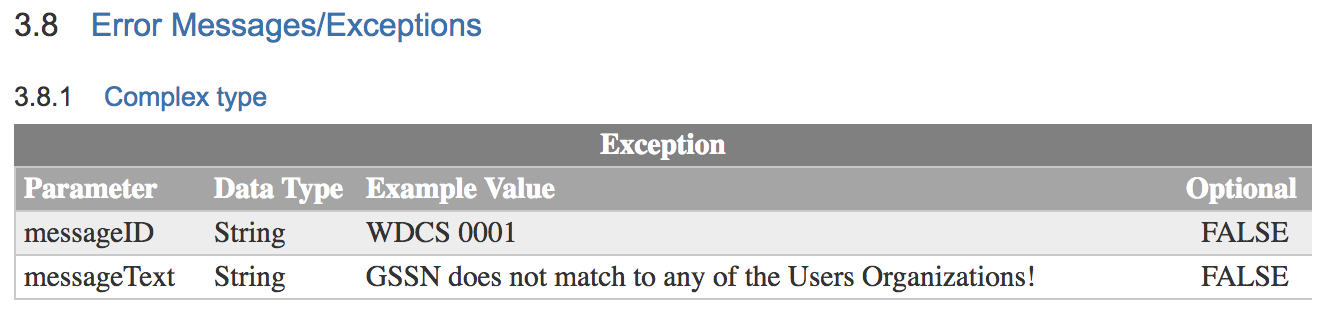
\includegraphics[keepaspectratio,alt={the document}]{images/about_comments_1.png}}

那么问题来了，这和代码定义完全不一样啊！然后告诉我以代码为准。从这个代码根本无法确定错误返回结构。然后又看看我们这个模拟的stub的代码，关于出错的地方是这么定义的：

\begin{Shaded}
\begin{Highlighting}[]
\KeywordTok{public} \KeywordTok{class}\NormalTok{ OabResponseDto }\OperatorTok{\{}

    \KeywordTok{private} \DataTypeTok{boolean}\NormalTok{ success}\OperatorTok{;}

    \KeywordTok{private} \BuiltInTok{Object}\NormalTok{ result}\OperatorTok{;}

    \KeywordTok{private} \BuiltInTok{String}\NormalTok{ error}\OperatorTok{;}
\end{Highlighting}
\end{Shaded}

后来才觉察到，这是另一个系统的接口返回了。但几个系统的模拟stub都写到了一起，让人完全无法确定真实的三方接口定义。最终，我找到了调用这个接口的测试环境，自己调用了一次，原来结果是这样的：

\begin{Shaded}
\begin{Highlighting}[]
\OperatorTok{\{}\StringTok{"error"}\OperatorTok{:\{}\StringTok{"errorCode"}\OperatorTok{:}\StringTok{"WDCS0003"}\OperatorTok{,}\StringTok{"errorDesc"}\OperatorTok{:}\StringTok{"Resource not available!"}\OperatorTok{\}\}}
\end{Highlighting}
\end{Shaded}

这耗费了我半天的时间。于是为了避免有人再踩这种坑，我加了个注释在这里：

\begin{Shaded}
\begin{Highlighting}[]
\NormalTok{Fallback }\FunctionTok{generateFallback}\OperatorTok{(}\BuiltInTok{String}\NormalTok{ message}\OperatorTok{)} \OperatorTok{\{}
    \ControlFlowTok{try} \OperatorTok{\{}
        \CommentTok{/**}
         \CommentTok{*}\NormalTok{ example actual response from eva}\CommentTok{:}
         \CommentTok{*} \CommentTok{\{"}\NormalTok{error}\CommentTok{":\{"}\NormalTok{errorCode}\CommentTok{":"}\NormalTok{WDCS0003}\CommentTok{","}\NormalTok{errorDesc}\CommentTok{":"}\NormalTok{Resource not available}\CommentTok{!"\}\}}
         \CommentTok{*/}
        \DataTypeTok{int}\NormalTok{ startPos }\OperatorTok{=}\NormalTok{ message}\OperatorTok{.}\FunctionTok{indexOf}\OperatorTok{(}\StringTok{"\{}\SpecialCharTok{\textbackslash{}"}\StringTok{error}\SpecialCharTok{\textbackslash{}"}\StringTok{:"}\OperatorTok{);}
\end{Highlighting}
\end{Shaded}

然而这又被批判了，理由是这段注释不能解释代码。因为这里message并不是这样。那message到底是什么样？他们说，你可以调试打个断点看。难道让每一个看代码的人都打个断点来看么，这是什么逻辑！我就呵呵了。最终我还是妥协了，删了呗，对我而言无任何影响。


\end{document}
